\documentclass{standalone}
\begin{document} 

\subsection{Aufgabe 4.9}

\begin{enumerate}[a)]
    \item $M_1 = \{ (x,y)^T \in \mathbb{R}^2 \mid \abs{x} + \abs{y} \leq 1 \}$
    \begin{figure}[htbp]
        \centering
        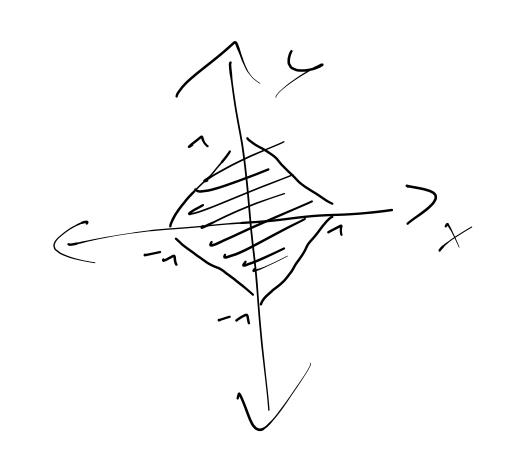
\includegraphics[width=8cm]{4_9_a}
    \end{figure}
    \FloatBarrier

    \item $M_1 = \{ (x,y)^T \in \mathbb{R}^2 \mid x^2 + y^2 > 1 \}$
    \begin{figure}[htbp]
        \centering
        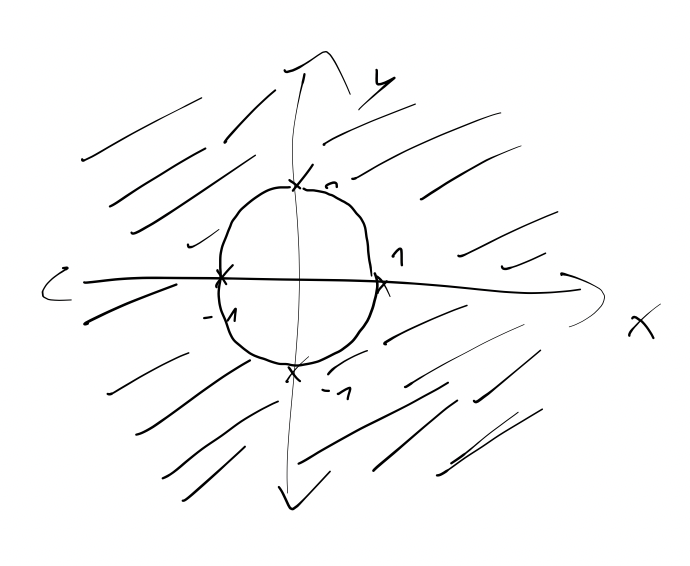
\includegraphics[width=8cm]{4_9_b}
    \end{figure}
    \FloatBarrier
    
    \item $M_1 = \{ (x,y)^T \in \mathbb{R}^2 \mid \max\{x,y\} \leq 1 \}$
    \begin{figure}[htbp]
        \centering
        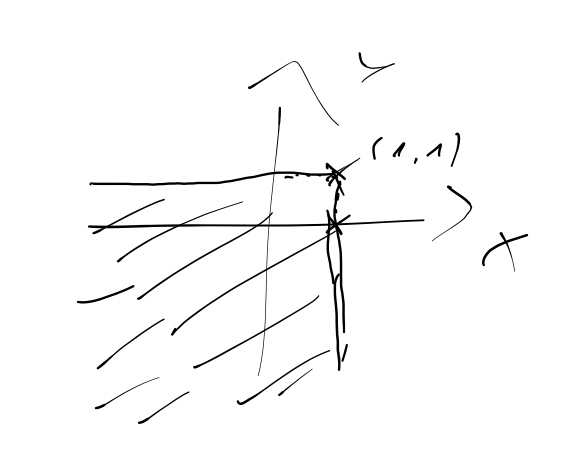
\includegraphics[width=8cm]{4_9_c}
    \end{figure}
    \FloatBarrier
\end{enumerate}

\subsection{Aufgabe 4.10}
% Hier eure Lösung eingeben
$$x_0 \in \mathbb{R} \text{, } A(x_0) \text{ gilt für } x < x_0$$
\begin{enumerate}[a)]
    \item $x =\frac{1}{2}x_0$ - gilt nicht, da $x_0$ negativ sein könnte
    \item $x =x_0 - 3$ - gilt nicht, da $x_0 - 3 < x_0$
    \item $y^2 < x_0$, bzw. $-\sqrt{x_0} < y < +\sqrt{x_0}$ für $x_0 \geq 0$. Wenn $x_0 < 0$ ist, existiert ein solches reelles $y$ nicht.
    \item \begin{align}
        \abs{y+2} &< x_0 \\
        y+2 > 0 &\vee y+2 < 0 \\
        y > -2 &\vee y < -2 \\
        \\
        y+2 < x_0 &\vee y+2 > x_0 \\
        y < x_0 -2 &\vee y > x_0 -2 \\
        \mathbb{L}_1 = ]-2,x_0 -2[ &\vee \mathbb{L}_2 = ]x_0-2, -2[
    \end{align}
    Es existiert kein $x_0$, für das beide Bedingungen erfüllt sind.
    Für $x_0 < 0$ gilt $\mathbb{L} = \mathbb{L}_2$ und andersherum.
\end{enumerate}

\subsection{Aufgabe 4.11}
% Hier eure Lösung eingeben
$$\abs{x^2 - 9} < \abs{x-1}$$
\begin{itemize}
    \item Fall 1: $x-1 > 0 \Leftrightarrow x > 1$\begin{align}
        \abs{x^2 - 9} &< x-1 
    \end{align}
    \item Fall 1.1: $x^2-9 > 0 \Leftrightarrow -3 > x > 3$\begin{align}
        x^2 - 9 &< x - 1 \\
        x^2 - x - 8 &< 0 \\
        (x-\frac{1}{2})^2 &< \frac{33}{4}
    \end{align}
    \item Fall 1.1.1: $x-\frac{1}{2} > 0 \Leftrightarrow x > \frac{1}{2}$\begin{align}
        x-\frac{1}{2} &< \frac{\sqrt{33}}{2} \\
        x &< \frac{1}{2} + \frac{\sqrt{33}}{2} \approx 3.37
        \Rightarrow \mathbb{L}_{1.1.1} = (\frac{1}{2}, 3.37)
    \end{align}
    \item Fall 1.1.2: $x-\frac{1}{2} \leq 0 \Leftrightarrow x \leq \frac{1}{2}$\begin{align}
        x-\frac{1}{2} > -\frac{\sqrt{33}}{2} \\
        x > \frac{1}{2} - \frac{\sqrt{33}}{2} \approx -2.37 \\
        \Rightarrow \mathbb{L}_{1.1.2} = (-2.37,\frac{1}{2}] \\
        \Rightarrow \mathbb{L}_{1.1} = (3, 3.37)
    \end{align}
    \item Fall 1.2: $x^2-9 \leq 0 \Leftrightarrow -3 \leq x \leq 3$\begin{align}
        x^2 - 9 &> 1-x \\
        x^2 + x -10 &> 0 \\
        (x+\frac{1}{2})^2 -\frac{41}{4} &> 0
    \end{align}
    \item Fall 1.2.1: $x+\frac{1}{2} > 0 \Leftrightarrow x > -\frac{1}{2}$\begin{align}
        x > -\frac{1}{2}+\frac{\sqrt{41}}{2} \approx 2.7
    \end{align}
    \item Fall 1.2.2: $x+\frac{1}{2} \leq 0 \Leftrightarrow x \leq -\frac{1}{2}$\begin{align}
        x < -\frac{1}{2}-\frac{\sqrt{41}}{2} \approx -3.7 \\
        \Rightarrow \mathbb{L}_{1.2} = (2.7, 3] \\
        \Rightarrow \mathbb{L}_{1} = (2.7, 3.37)
    \end{align}

    \item Fall 2: $x-1 \leq 0 \Leftrightarrow x \leq 1$\begin{align}
        \abs{x^2 - 9} &< 1-x
    \end{align}
    \item Fall 2.1: $x^2-9 > 0 \Leftrightarrow -3 > x > 3$\begin{align}
        x^2 - 9 &< 1 - x \\
        x^2 + x - 10 &< 0 \\
        (x+\frac{1}{2})^2 &< \frac{41}{4}
    \end{align}
    \item Fall 2.1.1: $x+\frac{1}{2} > 0 \Leftrightarrow x > -\frac{1}{2}$\begin{align}
        x+\frac{1}{2} &< \frac{\sqrt{41}}{2} \\
        x &< -\frac{1}{2} + \frac{\sqrt{41}}{2} \approx 2.7
    \end{align}
    \item Fall 2.1.2: $x+\frac{1}{2} \leq 0 \Leftrightarrow x \leq -\frac{1}{2}$\begin{align}
        x+\frac{1}{2} &> -\frac{\sqrt{41}}{2}\\
        x &> -\frac{1}{2} - \frac{\sqrt{41}}{2} \approx -3.7
        \Rightarrow \mathbb{L}_{2.1} = (-3.7,-3]
    \end{align}
    \item Fall 2.2: $x^2-9 \leq 0 \Leftrightarrow -3 \leq x \leq 3$\begin{align}
        x^2 - 9 &< x-1 \\
        x^2 - x -8 &< 0 \\
        (x-\frac{1}{2})^2 -\frac{33}{4} &> 0
    \end{align}
    \item Fall 2.2.1: $x-\frac{1}{2} > 0 \Leftrightarrow x > \frac{1}{2}$\begin{align}
        x > \frac{1}{2}+\frac{\sqrt{33}}{2} \approx 3.37
    \end{align}
    \item Fall 2.2.2: $x-\frac{1}{2} \leq 0 \Leftrightarrow x \leq \frac{1}{2}$\begin{align}
        x < \frac{1}{2}-\frac{\sqrt{33}}{2} \approx -2.37 \\
        \Rightarrow \mathbb{L}_{2.2} = [-3,-2.37)
        \Rightarrow \mathbb{L}_{2} = (-3.7,-2.37)
        \Rightarrow \mathbb{L} = (-3.7,-2.37) \cup (2.37,3.37)
    \end{align}


\end{itemize}

\subsection{Aufgabe 4.12}
% Hier eure Lösung eingeben
\begin{align}
    (ab + cd)^2 &\leq (a^2 + c^2)(b^2 + d^2) \\
    (ab)^2 + (cd)^2 + 2abcd &\leq (ab)^2 + (ad)^2 + (cb^2) + (cd)^2 \\
    2abcd &\leq (ad)^2 + (cb)^2 \text{, mit } ad = x \text{ und } cb = y\\
    2xy &\leq x^2 + y^2 \\
    0 &\leq x^2-2xy+y^2 \\
    0 &\leq (x-y)^2 \text{, das ist wahr}
\end{align}
\end{document}